\documentclass{article}
\usepackage[utf8]{inputenc}
\usepackage{graphicx}
\usepackage[paper=a4paper,left=3cm, right=3cm, top=2cm]{geometry}
\usepackage{blindtext}
\usepackage{multicol}
\usepackage{pgfplots}
\usepackage{float}
\usepackage{biblatex} %Imports biblatex package
\usepackage{amsmath}
\addbibresource{ai.bib} %Import the bibliography file

 
\pgfplotsset{compat = newest}

\title{\textbf{An Analysis of $L_2$ and Dropout Regularization in a Simple Neural Network}}
\author{Neelkant Newra \\ \textit{Department of Biomedical Engineering} \\ National Institute of Technology, Raipur \\ Email: newra008@gmail.com}
\date{November 2021}

\begin{document}

\maketitle

\begin{abstract}\textbf{
    In supervised learning our main initiative is to avoid over-fitting issue. Over-fitting usually occurs when we have lots of unnecessary landmark detected by model or detection of false parameter. This are also due to the complex learning algorithm or in our case a large neural network. A typical approach to solve this problems are to provide a large penalty or dropping some unit in hidden layer while training, it is known as regularization. In this paper we  will discuss about different regularization technique and give an analysis of $L_2$-norm or Ridge Regression and dropout in single hidden layer neural network.} \\ \\
    \textbf{\textit{Keywords- neural network; over-fitting;regularization;perceptrons;dropout,$L_2$-norms}}
\end{abstract}

\begin{multicols}{2}
\section{Introduction}
The fundamental aim of supervised learning is to get a satisfactory outcome not only in the training set, but also in the development set. Our goal isn't just to reproduce the pattern perfectly; we want to comprehend it and develop a model that can perform properly with other patterns as well\cite{7877209}. Assume we have a model for a basic polynomial regression problem in which we would fit a set of $m$ data point, it is arranged in $\{{x^{(i)},y^{(i)}}\}$ where $i$ varies from $1,2,3 ... m $, we are minimizing sum of squared error cost function or (RMSE)root mean squared error cost function. For the purpose of simplicity we will take MSE(mean squared error). This problem may alternatively be thought of as translating a function with $x$ to an output $y$ or $y=f(x)$. Suppose we have $P \ coordinate$ following $(0,0),(0.3,0.3),(0.5,2),(1,3),(2,3),(2,2)$, $(2.5,3.5),(3,3),(4,4)$. Figure 1 shows that the poor generalisation can lead to the under-fitting issue if we get very few coefficients represented by red line, where we are missing most of the coordinate. On the other hand, having a large number of coefficients might lead to poor generalisation since we are over-fitting the data point, and there is a significant possibility that the accuracy will not be the same for test data.
%---------------------- figure 1 plotting -----------------
\begin{figure}[H]
\label{fig:1}
    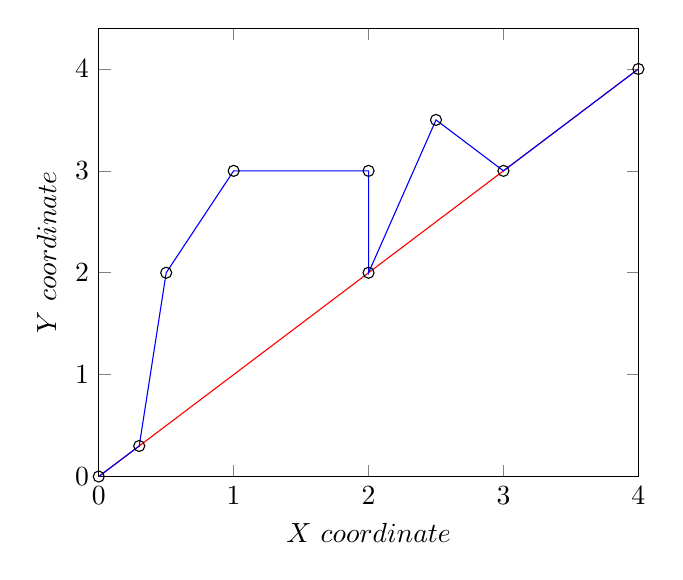
\begin{tikzpicture}
        \begin{axis}[
        xlabel=$X \  coordinate$,
        ylabel=$Y \ coordinate$,
        xmin = 0,
        xmax = 4,
        ymin=0]
            \addplot[red] {x};
            \addplot[color = blue, mark color = red]
     coordinates{
    (0,0) (0.3,0.3) (0.5,2) (1,3) (2,3) (2,2) (2.5,3.5) (3,3) (4,4)
        }; 
        \addplot[only marks, mark=o, color = black]
        coordinates{
    (0,0) (0.3,0.3) (0.5,2) (1,3) (2,3) (2,2) (2.5,3.5) (3,3) (4,4)
        }; 
        \end{axis}
    \end{tikzpicture}
    \caption{Graph showing the over-fitting and under-fitting issue, where red line indicate the under-fitting problem where most of the coordinate missed, while blue line is showing over-fitting issue where the function is complex and fitting all the coordinate.}
  \end{figure}
  
 %------------------------ figure 1 completed --------------------------
  
In this paper, we will examine the over-fitting problem, which is also represented as a blue line in Figure \ref{fig:1}, and attempt to solve the problem using various regularisation approaches. We will be using most used regularization method $L_2 \ regularisation$ and $Dropout$ for this. $Dropout$ has recently gain more advantage as it has given a significant result in the highly dense neural network. 

Lets take a practical example of pneumonia detection using CXR(Chest X-ray). Suppose there are some images of patient having tumour and wear ornament. It is huge possibility that the model will over-fit for the necklace parameter which is absolutely wrong. 

One of the most widely used learning algorithm is Neural Network which is inspired by biological neuron, Where each dendrite can be refer as the input parameter and axon as the processed output. Multi Layer Perceptrons(MLPs) are a basic type of this network that feed-forwards from an input layer to zero or more hidden layers, then to an output layer. MLPs allow to process data in unidirectional, passing the value of one layer to another. In each layer it is connected with highly dense interconnected simple or complex processing element which is also called neuron. The MLPs have successfully involved in solving the complex problem in the are of medical, digit recognition, sign language recognition, face detection, object detection, market price prediction, Recommender systems etc. The input and output dimensions of a neural network are determined by the objectives, such as how many parameters you choose to feed for processing and how many parameters you want as an output. If you're conducting multitask learning, you can have multiple outputs. The number of hidden layer and neuron in each hidden layer are free parameter that can be chosen based on the model we select for particular problem. The number of layer and number of neuron defined the neural architecture whether is it is shallow or densed. More the network is densed more near coefficient we get. In most of the case dense neural network is used if the problem is to complex, mostly problem related with images. Denser the network more the computational requirement. Generally while dealing with highly densed neural network it is huge chances that the model will get over-fitted. So some paper suggested the method of addition of penalty or regularization term to avoid this over-fitting controlling the model parameter. We have $L_2 \ regularization$ which is widely used in machine learning community also known as ridge regularization (more generally Tikhonov’s regularization)\cite{NIPS2011_33ceb07b}. We have one more approach which recently gain fame as complexity of neural network keeps increasing, the method is $dropout$ in which layer of neuron are dropped in random or fixed pattern. As the neuron drop the layer become less dense and reduce the effect of over-fitting. In this paper we will study the effect of $L_2 \ regularization$ and $dropout$ in a single hidden layer neural network. We will compare it on the basis of various parameter like accuracy, F1 score, precision etc. Before we go any further, let's have a look at a simple neuron with one hidden layer and learn about its various components.
%---------------------- figure 2 plotting -----------------
\begin{figure}[H]
\label{fig:2}
   \tikzset{%
  every neuron/.style={
    circle,
    draw,
    minimum size=1cm
  },
  neuron missing/.style={
    draw=none, 
    scale=4,
    text height=0.333cm,
    execute at begin node=\color{black}$\vdots$
  },
}

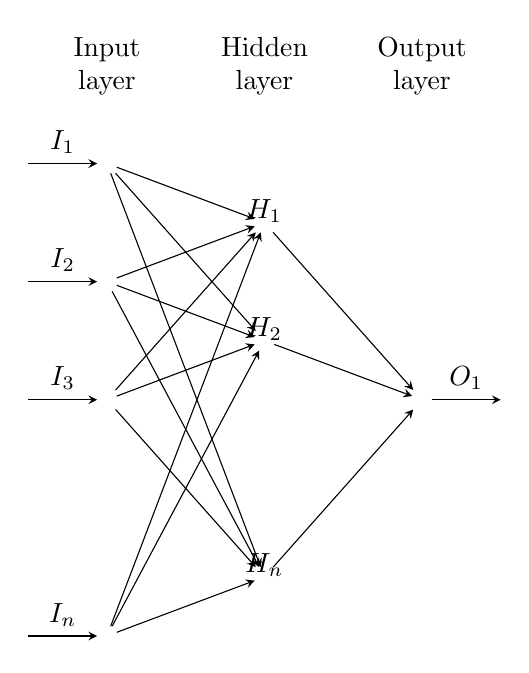
\begin{tikzpicture}[x=1cm, y=1.5cm, >=stealth]

\foreach \m/\l [count=\y] in {1,2,3,missing,4}
  \node [every neuron/.try, neuron \m/.try] (input-\m) at (0,2.5-\y) {};

\foreach \m [count=\y] in {1,2,missing,3}
  \node [every neuron/.try, neuron \m/.try ] (hidden-\m) at (2,2-\y*1) {};

\foreach \m [count=\y] in {1}
  \node [every neuron/.try, neuron \m/.try ] (output-\m) at (4,0.5-\y) {};

\foreach \l [count=\i] in {1,2,3,n}
  \draw [<-] (input-\i) -- ++(-1,0)
    node [above, midway] {$I_\l$};

\foreach \l [count=\i] in {1,2,n}
  \node [above] at (hidden-\i.south) {$H_\l$};

\foreach \l [count=\i] in {1}
  \draw [->] (output-\i) -- ++(1,0)
    node [above, midway] {$O_\l$};

\foreach \i in {1,...,4}
  \foreach \j in {1,...,3}
    \draw [->] (input-\i) -- (hidden-\j);

\foreach \i in {1,...,3}
  \foreach \j in {1}
    \draw [->] (hidden-\i) -- (output-\j);

\foreach \l [count=\x from 0] in {Input, Hidden, Output}
  \node [align=center, above] at (\x*2,2) {\l \\ layer};

\end{tikzpicture}
    \caption{Figure showing the input, hidden and output layer in a neural network. Where input layer consist of n input, we have 1 hidden layer consisting of n neuron interconnected and output layer consist of 1 output neuron. }
  \end{figure}
%------------------------ figure 2 completed --------------------------
In this research we will try to achieve the benefit of various regularization method, as the first section was a brief introduction on over-fitting issue and a simple concept of neural network. In the second section we will discuss $L_2 \ regularization$ and $Dropout$ in much detail. With the help of the above neural network architecture[Figure \ref{fig:2}], we will look at a few examples.. Then we'll discuss about the dataset we'll be testing with, which is the MNIST dataset on Kaggle\cite{lecun-mnisthandwrittendigit-2010}. In section four, we will evaluate the accuracy of several neural networks on $L_2 \ regularization$ and $Dropout$.
\section{$L_2 \ norm \  and\  Dropout$}
Since $L_2 \ norm$ is widely used in ML community it is also simply refer as Regularization. In $L_2 \ norm$ we add an addition term which act as penalty and due to which the weight of parameter decreases, due to the decay in weight $L_2 \ regularization$ is some time refer as simply weight decay.\cite{martin2018implicit} Before looking for its effect in neural network let's see how it act for Logistic regression problem. The cost function for $L_2 \ normalized$ logistic regression model is: \\

\begin{equation}
\label{eq:1}
J(W,b) = {1 \over m} \sum _{i=1}^m L(\hat y^{(i)},y^{(i)}) + {\lambda \over 2m} ||W||_2^2 + {\lambda \over 2m} b^2
\end{equation}
\begin{equation}
\label{eq:2}
    ||W||_2^2 = \sum_{j=1}^{n_x} W_j^2 = W^TW
\end{equation}
\\
here, $\lambda$ is the regularization parameter which we can tuned as per the given set of data. We will see the effect of increase and decrease when we implement $L_2 \ norm$ in Neural Network. In the Equation \ref{eq:1} we see the biased term $b$ which is constant term and doesn't have a significant effect in cost function if we goes for higher value for Weighted term, so in this paper we will omit $b$. Equation \ref{eq:2} shows the value of the penalty or $L_2 \ regularization$ also known as $Euclidean \ norms$. As we are familiar on how a logistic regression can me normalized, so let us implement it in on a neural network consisting of $l$ weighted parameter and coefficient.
\begin{equation}
\label{eq:3}
\begin{aligned}
    J([W^{[1]},b^{[1]},...,W^{[l]},b^{[l]}]) = 
    {1 \over m} \sum _{i=1}^m L(\hat y^{(i)},y^{(i)})\\+{\lambda \over 2m} \sum_{p=1}^{l}||W^{[p]}||_F^2
    \end{aligned}
\end{equation}
where, \\
\begin{equation}
\label{eq:4}
    || W^{[l]}||^2_F = \sum_{i=1}^{n^{[l]}} \sum_{j=1}^{n^{[l-1]}} (W_{ij}^{[l]})^2
\end{equation}
\\
here, Equation \ref{eq:3} represent the normalised equitation for Neural Network, where $m$ is the training examples, $\lambda$ is the hyper-parameter  $\hat y^{(i)}$ is the prediction by the model and $y^{(i)}$ is the actual value. Equation \ref{eq:4} is also known as Frobenius norm sometime also refer as Euclidean norms. Let us assume that $H_x$ is the value obtain from the back propagation so,
\begin{equation}
\label{eq:5}
    dW^{[l]} = H_x + {\lambda \over m } W^{[l]}
\end{equation}
\begin{equation}
\label{eq:6}
    W^{[l]} = W^{l} - \alpha dW^{[l]}
\end{equation}

Taking Reference of equation \ref{eq:6} we can say that weight is decaying as we are subtracting $dW$ parameter and in equation \ref{eq:5} we can see an addition frobenius norm term which is increasing the value of $dW^{[l]}$ thus decrease the value of $W^{[l]}$. So as the value of $\lambda$ increase the value of $W^{[l]}$ decreases. Let us look at the graph of $tanh$ activation function and try to understand the effect of decreasing $W^{[l]}$. 

%---------------------- figure 3 plotting -----------------
\begin{figure}[H]
\label{fig:3}
    \begin{tikzpicture}
        \begin{axis}[
        xticklabel=\empty,yticklabel=\empty,minor tick num=1,
        axis lines = middle,
        xlabel=$z$,
        ylabel=$g(z)$]
            \addplot[red] {tanh(x)};
            \addplot[blue] coordinates{
    (-1,-0.90514825364) (1,0.90514825364)
        };
        \end{axis}
    \end{tikzpicture}
    \caption{In the graph the red line shows the $tanh$ activation function graph and blue line represent the portion at which act as linear.}
  \end{figure}
  
 %------------------------ figure 3 completed --------------------------
 
 We know that:
\begin{equation}
\label{eq:7}
    g(Z) = tanh(Z)
\end{equation}
\begin{equation}
\label{eq:8}
    Z^{[l]} = W^{[l]}a^{[l-1]} + b^{[l]}
\end{equation}

from equation \ref{eq:7} and equation \ref{eq:8} we can say that when the value of $W^[l]$ decreases $g(Z)$ tends more toward the linear, We can see this in Figure \ref{fig:3} where blue line represent the line where we have optimised value for $g(Z)$, which reducing the complexity of regression or classification model and makes our model little biased. We will look the same intuition when we talk about the dropout which have some conceptual similarity with the same which we learnt above.

We have $Dropout$ as another regularization method which is highly used in many research paper where highly complex neural network is used. Previous research paper suggest $Dropout$ has managed to give very good accuracy and is highly optimised to reduce the computational cost of any model. Drop out is method of regularization in which we drop neurons in any hidden layer. As we drop one neuron the corresponding connection of the neuron get decomposed. So we can alternatively says that it is creating some new network architecture each time it drops the neuron in any hidden layer. 

\section{Method}

In this experiment we will be using famous MNIST data-set which contains 70000 handwritten digit images of shape 28x28 flatten and arranged in 784 pixel column and a label column. pixel value varies from 0-255 while label  value varies from 0-1 integer value. We will be using 60,000 images for training 5,000 for validation while 5,000 for testing. Each image is already normalised and well centered. 

\begin{figure}[H]
    \centering
    \includegraphics[width=6cm]{images/images.png}
    \caption{Images from Kaggle MNIST Digit recogniser Data-set, 25 randomly selected handwritten digit}
    \label{fig:4}
\end{figure}

\begin{figure}[H]
    \centering
    \includegraphics[width=6cm]{images/img1.png}
    \caption{Images converted to binary images as color has no significance.}
    \label{fig:5}
\end{figure}

The Data-set consist of BGR images as shown in Figure \ref{fig:4} but since color has no additional significance it is thus converted to binary images as shown in Figure \ref{fig:5} with each pixel values either 0 or 1 where 0 represent black and 1 represent white.

So, let's look at neural network structure, it consist of $L$ layers where $L$ varies as $\{0,1,2,...,L-1\}$ let's $l$ be the indexing of the layers where $l=0$ state the input layer while $l = L-1$  output layer. We know that in Neural network we feed forward the processing so assume $l$ layer has input vector $z^{(l)}$ and $y^{(l)}$ is the output vector of $l$ layer. Where we have $W^{(l)}$ and $b^{(l)}$ as weight and biased term of that particular layer. So we know that the initial layer is input and final layer is output, so the layer in between is the hidden layer. So the hidden layer start from index 1 and end at index L-1. Let us look at the output of a hidden layer:

\begin{equation}
\label{eq:9}
    z^{(l+1)} =W^{(l+1)}y^{(l)} + b^{(l+1)}
\end{equation}
\begin{equation}
\label{eq:10}
    y^{(l+1)} =a(z^{(l+1)})
\end{equation}

Where in equation \ref{eq:10} $a(.)$ represent the activation function. Let's apply dropout in the equation \ref{eq:9} and equation \ref{eq:10}:
\begin{equation}
\label{eq:11}
    \delta_i^{(l)} \sim Bernoulli(p)
\end{equation}
\begin{equation}
\label{eq:12}
    \tilde{y}^{(l)} = \delta^{(l)} \otimes y^{(l)}
\end{equation}
\begin{equation}
\label{eq:13}
     z^{(l+1)} =W^{(l+1)}\tilde{y}^{(l)} + b^{(l+1)}
\end{equation}
\begin{equation}
\label{eq:14}
    y^{(l+1)} =a(z^{(l+1)})
\end{equation}

The equation \ref{eq:9},equation \ref{eq:10},equation \ref{eq:11},equation \ref{eq:12},equation \ref{eq:13},equation \ref{eq:14} are taken from \cite{7877209}. Where $\otimes$ in equation \ref{eq:12} represent the element-wise product. if you want to look more for bernoulli random varible refer Article \cite{https://doi.org/10.1002/bimj.201500115}. 

Now Let us look at some experimental result shown in Table 1 where we see that Drop-out has given us the significance accuracy in case of single neural network as we increase the neuron in hidden layer. In the table the value are in percentage accuracy. 

\begin{table}[H]
    \centering
    \begin{tabular}{|p{2 cm}|c|c|c|}
    \hline
    \centering Neuron Used & 
         \centering $L_2 \ regularization$
         & Dropout \\
    \hline
    100
    &  96.97
    &  96.51 \\
    200
    &  97.02
    &  97.49 \\
    300
    &  97.05
    &  97.82 \\
    400
    &  97.05
    &  97.97 \\
    500
    &  96.90
    &  97.99 \\
    600
    &  96.99
    &  98.09 \\
    700
    &  96.96
    &  98.19 \\
    800
    &  96.86
    &  98.29 \\
    900
    &  96.91
    &  98.22 \\
    1000
    &  96.61
    &  98.17 \\
    \hline
    
    \end{tabular}
    \caption{Classification performance between $L_2 \ regularization$ and $Dropout$ on MNIST Dataset Where Neuron used are Integer while the other numerical value is in percentage\cite{7877209}}
    \label{tab:my_label}
\end{table}

The Table \ref{tab:my_label}  shows that We see an inconsistency in $L_2 \ regularization$ as the neuron used increased the highest accuracy in $L_2 \ regularization$ is achieve when we keep the neuron size at 300-400, While on the other case in dropout we achieve that much accuracy at 200 neuron, Although the highest accuracy in $Dropout$ is seen to be at neuron size 800. So We can say that as the neuron size increases the drop out shows a good accuracy. 

\section{Conclusion}

$Dropout$ is very new to the Machine Learning Community in term of use, Dropping the neuron cost less computation compare to penalizing. Since, neuron is dropped it has no dependency on previous or forth neuron. That is the main reason we see a very good accuracy for the dropout as the neuron size increases. While we see a satisfactory result for $L_2 \ regularization$ for lower neuron size. But in contrast to accuracy the precision of $L_2 \ regularization$ is higher compare to $Dropout$. The experimental result are taken from \cite{7877209} and verified with MNIST Data-set. For the further research work we can include more coloured imaged data-set and verify the same for them.

\end{multicols}


\printbibliography

\end{document}

